\documentclass[twoside]{book}

% Packages required by doxygen
\usepackage{calc}
\usepackage{doxygen}
\usepackage{graphicx}
\usepackage[utf8]{inputenc}
\usepackage{makeidx}
\usepackage{multicol}
\usepackage{multirow}
\usepackage{textcomp}
\usepackage[table]{xcolor}

% Font selection
\usepackage[T1]{fontenc}
\usepackage{mathptmx}
\usepackage[scaled=.90]{helvet}
\usepackage{courier}
\usepackage{amssymb}
\usepackage{sectsty}
\renewcommand{\familydefault}{\sfdefault}
\allsectionsfont{%
  \fontseries{bc}\selectfont%
  \color{darkgray}%
}
\renewcommand{\DoxyLabelFont}{%
  \fontseries{bc}\selectfont%
  \color{darkgray}%
}

% Page & text layout
\usepackage{geometry}
\geometry{%
  a4paper,%
  top=2.5cm,%
  bottom=2.5cm,%
  left=2.5cm,%
  right=2.5cm%
}
\tolerance=750
\hfuzz=15pt
\hbadness=750
\setlength{\emergencystretch}{15pt}
\setlength{\parindent}{0cm}
\setlength{\parskip}{0.2cm}
\makeatletter
\renewcommand{\paragraph}{%
  \@startsection{paragraph}{4}{0ex}{-1.0ex}{1.0ex}{%
    \normalfont\normalsize\bfseries\SS@parafont%
  }%
}
\renewcommand{\subparagraph}{%
  \@startsection{subparagraph}{5}{0ex}{-1.0ex}{1.0ex}{%
    \normalfont\normalsize\bfseries\SS@subparafont%
  }%
}
\makeatother

% Headers & footers
\usepackage{fancyhdr}
\pagestyle{fancyplain}
\fancyhead[LE]{\fancyplain{}{\bfseries\thepage}}
\fancyhead[CE]{\fancyplain{}{}}
\fancyhead[RE]{\fancyplain{}{\bfseries\leftmark}}
\fancyhead[LO]{\fancyplain{}{\bfseries\rightmark}}
\fancyhead[CO]{\fancyplain{}{}}
\fancyhead[RO]{\fancyplain{}{\bfseries\thepage}}
\fancyfoot[LE]{\fancyplain{}{}}
\fancyfoot[CE]{\fancyplain{}{}}
\fancyfoot[RE]{\fancyplain{}{\bfseries\scriptsize Generated on Mon Feb 8 2016 14\-:01\-:15 for Driver\-Tcp\-Socket\-Driver by Doxygen }}
\fancyfoot[LO]{\fancyplain{}{\bfseries\scriptsize Generated on Mon Feb 8 2016 14\-:01\-:15 for Driver\-Tcp\-Socket\-Driver by Doxygen }}
\fancyfoot[CO]{\fancyplain{}{}}
\fancyfoot[RO]{\fancyplain{}{}}
\renewcommand{\footrulewidth}{0.4pt}
\renewcommand{\chaptermark}[1]{%
  \markboth{#1}{}%
}
\renewcommand{\sectionmark}[1]{%
  \markright{\thesection\ #1}%
}

% Indices & bibliography
\usepackage{natbib}
\usepackage[titles]{tocloft}
\setcounter{tocdepth}{3}
\setcounter{secnumdepth}{5}
\makeindex

% Hyperlinks (required, but should be loaded last)
\usepackage{ifpdf}
\ifpdf
  \usepackage[pdftex,pagebackref=true]{hyperref}
\else
  \usepackage[ps2pdf,pagebackref=true]{hyperref}
\fi
\hypersetup{%
  colorlinks=true,%
  linkcolor=blue,%
  citecolor=blue,%
  unicode%
}

% Custom commands
\newcommand{\clearemptydoublepage}{%
  \newpage{\pagestyle{empty}\cleardoublepage}%
}


%===== C O N T E N T S =====

\begin{document}

% Titlepage & ToC
\hypersetup{pageanchor=false}
\pagenumbering{roman}
\begin{titlepage}
\vspace*{7cm}
\begin{center}%
{\Large Driver\-Tcp\-Socket\-Driver }\\
\vspace*{1cm}
{\large Generated by Doxygen 1.8.6}\\
\vspace*{0.5cm}
{\small Mon Feb 8 2016 14:01:15}\\
\end{center}
\end{titlepage}
\clearemptydoublepage
\tableofcontents
\clearemptydoublepage
\pagenumbering{arabic}
\hypersetup{pageanchor=true}

%--- Begin generated contents ---
\chapter{File Index}
\section{File List}
Here is a list of all documented files with brief descriptions\-:\begin{DoxyCompactList}
\item\contentsline{section}{\hyperlink{Driver__TcpSocketDriver_8c}{Driver\-\_\-\-Tcp\-Socket\-Driver.\-c} \\*Source file of Tcp\-Socket\-Driver Service }{\pageref{Driver__TcpSocketDriver_8c}}{}
\end{DoxyCompactList}

\chapter{File Documentation}
\hypertarget{Driver__TcpSocketDriver_8c}{\section{Driver\-\_\-\-Tcp\-Socket\-Driver.\-c File Reference}
\label{Driver__TcpSocketDriver_8c}\index{Driver\-\_\-\-Tcp\-Socket\-Driver.\-c@{Driver\-\_\-\-Tcp\-Socket\-Driver.\-c}}
}


Source file of Tcp\-Socket\-Driver Service.  


{\ttfamily \#include \char`\"{}types.\-h\char`\"{}}\\*
{\ttfamily \#include \char`\"{}Library\-\_\-\-Std\-Lib.\-h\char`\"{}}\\*
{\ttfamily \#include \char`\"{}Driver\-\_\-\-Tcp\-Socket\-Driver.\-h\char`\"{}}\\*
{\ttfamily \#include $<$netinet/in.\-h$>$}\\*
{\ttfamily \#include $<$sys/socket.\-h$>$}\\*
{\ttfamily \#include $<$sys/types.\-h$>$}\\*
{\ttfamily \#include $<$sys/ioctl.\-h$>$}\\*
{\ttfamily \#include $<$unistd.\-h$>$}\\*
{\ttfamily \#include $<$netdb.\-h$>$}\\*
{\ttfamily \#include $<$fcntl.\-h$>$}\\*
{\ttfamily \#include $<$string.\-h$>$}\\*
{\ttfamily \#include $<$stdio.\-h$>$}\\*
{\ttfamily \#include $<$errno.\-h$>$}\\*
Include dependency graph for Driver\-\_\-\-Tcp\-Socket\-Driver.\-c\-:
\nopagebreak
\begin{figure}[H]
\begin{center}
\leavevmode
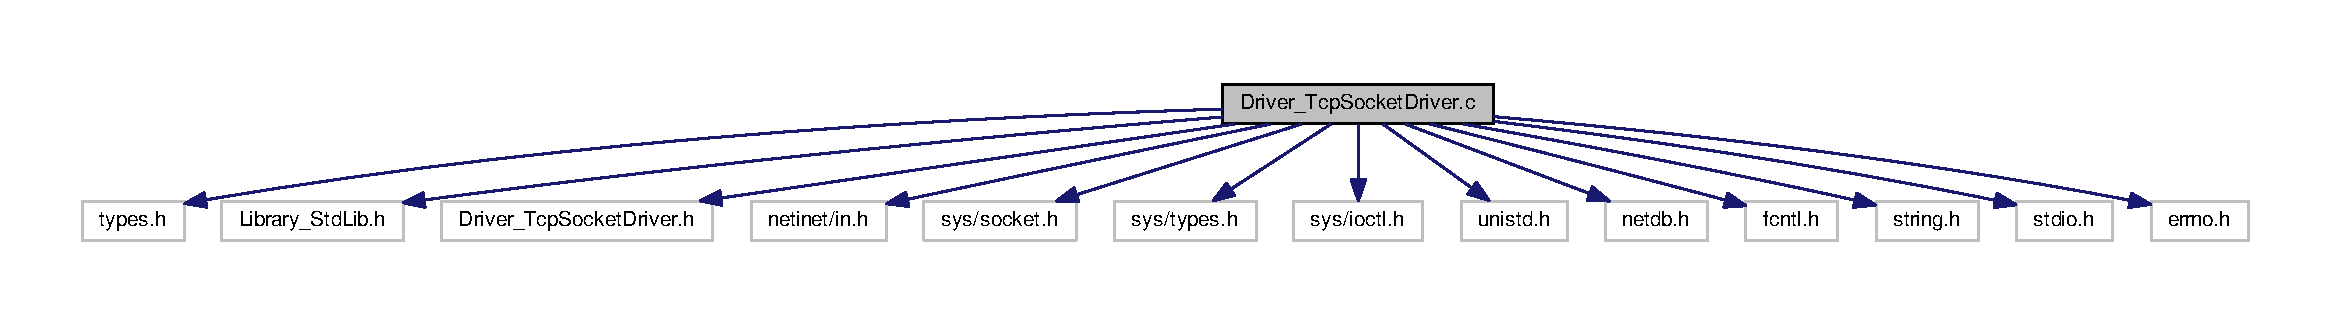
\includegraphics[width=350pt]{Driver__TcpSocketDriver_8c__incl}
\end{center}
\end{figure}
\subsection*{Functions}
\begin{DoxyCompactItemize}
\item 
Std\-\_\-\-Return\-Type \hyperlink{Driver__TcpSocketDriver_8c_ae4864de1aa2ccaa085ec95be15fdd514}{Drv\-Tcp\-Socket\-\_\-\-Initialize} (void)
\begin{DoxyCompactList}\small\item\em this function initializes internal variables \end{DoxyCompactList}\item 
Std\-\_\-\-Return\-Type \hyperlink{Driver__TcpSocketDriver_8c_a83e148a3b73c8a83dbf8d35c6b4676f9}{Drv\-Tcp\-Socket\-\_\-\-Open} (const Drv\-Tcpsocket\-\_\-cfg\-\_\-type $\ast$const pt\-\_\-configuration, Drv\-Tcpsocket\-\_\-descriptor\-\_\-type $\ast$const pt\-\_\-tcpsocket\-\_\-desc, E\-\_\-\-D\-R\-V\-T\-C\-P\-S\-O\-C\-K\-E\-T\-\_\-\-E\-R\-R\-O\-R $\ast$const pt\-\_\-error)
\begin{DoxyCompactList}\small\item\em this function opens tcp socket link \end{DoxyCompactList}\item 
Std\-\_\-\-Return\-Type \hyperlink{Driver__TcpSocketDriver_8c_a43a5289d8e2f1a4b36656cd6ec174a80}{Drv\-Tcp\-Socket\-\_\-\-Close} (Drv\-Tcpsocket\-\_\-descriptor\-\_\-type $\ast$const pt\-\_\-tcpsocket\-\_\-desc, E\-\_\-\-D\-R\-V\-T\-C\-P\-S\-O\-C\-K\-E\-T\-\_\-\-E\-R\-R\-O\-R $\ast$const pt\-\_\-error)
\begin{DoxyCompactList}\small\item\em this function closes link \end{DoxyCompactList}\item 
Std\-\_\-\-Return\-Type \hyperlink{Driver__TcpSocketDriver_8c_a6cc6b027de8d80500dbb1987bd27fdef}{Drv\-Tcp\-Socket\-\_\-\-Send} (const Drv\-Tcpsocket\-\_\-descriptor\-\_\-type t\-\_\-tcpsocket\-\_\-desc, const uint8 $\ast$const au8\-\_\-buffer, const uint32 u32\-\_\-buffer\-\_\-size, sint32 $\ast$const ps32\-\_\-written)
\item 
Std\-\_\-\-Return\-Type \hyperlink{Driver__TcpSocketDriver_8c_a056d8e2e3ee6d61985677dbf80be9a8b}{Drv\-Tcp\-Socket\-\_\-\-Receive} (const Drv\-Tcpsocket\-\_\-descriptor\-\_\-type t\-\_\-tcpsocket\-\_\-desc, const Drv\-Tcpsocket\-\_\-cfg\-\_\-type $\ast$const pt\-\_\-configuration, uint8 $\ast$const au8\-\_\-buffer, const uint32 u32\-\_\-buffer\-\_\-size, sint32 $\ast$const ps32\-\_\-read, E\-\_\-\-D\-R\-V\-T\-C\-P\-S\-O\-C\-K\-E\-T\-\_\-\-E\-R\-R\-O\-R $\ast$const pt\-\_\-error)
\begin{DoxyCompactList}\small\item\em this function reads datas from ethernet link \end{DoxyCompactList}\item 
Std\-\_\-\-Return\-Type \hyperlink{Driver__TcpSocketDriver_8c_a21cfd415598c17b7fd0e900421e12375}{Drv\-Tcp\-Socket\-\_\-\-Get\-\_\-\-Number\-Of\-Bytes} (const Drv\-Tcpsocket\-\_\-descriptor\-\_\-type t\-\_\-tcpsocket\-\_\-desc, uint32 $\ast$const pu32\-\_\-byte\-Size)
\begin{DoxyCompactList}\small\item\em this function gets the number of available data \end{DoxyCompactList}\end{DoxyCompactItemize}


\subsection{Detailed Description}
Source file of Tcp\-Socket\-Driver Service. \$\-Source\-: \hyperlink{Driver__TcpSocketDriver_8c}{Driver\-\_\-\-Tcp\-Socket\-Driver.\-c} \$\-Author\-: M\-Dega \$\-Date\-: 2015/12/30 

\subsection{Function Documentation}
\hypertarget{Driver__TcpSocketDriver_8c_a43a5289d8e2f1a4b36656cd6ec174a80}{\index{Driver\-\_\-\-Tcp\-Socket\-Driver.\-c@{Driver\-\_\-\-Tcp\-Socket\-Driver.\-c}!Drv\-Tcp\-Socket\-\_\-\-Close@{Drv\-Tcp\-Socket\-\_\-\-Close}}
\index{Drv\-Tcp\-Socket\-\_\-\-Close@{Drv\-Tcp\-Socket\-\_\-\-Close}!Driver_TcpSocketDriver.c@{Driver\-\_\-\-Tcp\-Socket\-Driver.\-c}}
\subsubsection[{Drv\-Tcp\-Socket\-\_\-\-Close}]{\setlength{\rightskip}{0pt plus 5cm}Std\-\_\-\-Return\-Type Drv\-Tcp\-Socket\-\_\-\-Close (
\begin{DoxyParamCaption}
\item[{Drv\-Tcpsocket\-\_\-descriptor\-\_\-type $\ast$const}]{pt\-\_\-tcpsocket\-\_\-desc, }
\item[{E\-\_\-\-D\-R\-V\-T\-C\-P\-S\-O\-C\-K\-E\-T\-\_\-\-E\-R\-R\-O\-R $\ast$const}]{pt\-\_\-error}
\end{DoxyParamCaption}
)}}\label{Driver__TcpSocketDriver_8c_a43a5289d8e2f1a4b36656cd6ec174a80}


this function closes link 


\begin{DoxyParams}{Parameters}
{\em pt\-\_\-tcpsocket\-\_\-desc} & \mbox{[}out\mbox{]} \-: link descriptor \\
\hline
{\em pt\-\_\-error} & \mbox{[}out\mbox{]} \-: Error type\\
\hline
\end{DoxyParams}
\begin{DoxyReturn}{Returns}
Std\-\_\-\-Return\-Type \-:
\begin{DoxyItemize}
\item E\-\_\-\-O\-K if good return function
\item E\-\_\-\-N\-O\-T\-\_\-\-O\-K if not 
\end{DoxyItemize}
\end{DoxyReturn}
Declaration

Initialization

Function Body

return code \hypertarget{Driver__TcpSocketDriver_8c_a21cfd415598c17b7fd0e900421e12375}{\index{Driver\-\_\-\-Tcp\-Socket\-Driver.\-c@{Driver\-\_\-\-Tcp\-Socket\-Driver.\-c}!Drv\-Tcp\-Socket\-\_\-\-Get\-\_\-\-Number\-Of\-Bytes@{Drv\-Tcp\-Socket\-\_\-\-Get\-\_\-\-Number\-Of\-Bytes}}
\index{Drv\-Tcp\-Socket\-\_\-\-Get\-\_\-\-Number\-Of\-Bytes@{Drv\-Tcp\-Socket\-\_\-\-Get\-\_\-\-Number\-Of\-Bytes}!Driver_TcpSocketDriver.c@{Driver\-\_\-\-Tcp\-Socket\-Driver.\-c}}
\subsubsection[{Drv\-Tcp\-Socket\-\_\-\-Get\-\_\-\-Number\-Of\-Bytes}]{\setlength{\rightskip}{0pt plus 5cm}Std\-\_\-\-Return\-Type Drv\-Tcp\-Socket\-\_\-\-Get\-\_\-\-Number\-Of\-Bytes (
\begin{DoxyParamCaption}
\item[{const Drv\-Tcpsocket\-\_\-descriptor\-\_\-type}]{t\-\_\-tcpsocket\-\_\-desc, }
\item[{uint32 $\ast$const}]{pu32\-\_\-byte\-Size}
\end{DoxyParamCaption}
)}}\label{Driver__TcpSocketDriver_8c_a21cfd415598c17b7fd0e900421e12375}


this function gets the number of available data 


\begin{DoxyParams}{Parameters}
{\em t\-\_\-tcpsocket\-\_\-desc} & \mbox{[}in\mbox{]} \-: Socket descriptor \\
\hline
{\em pu32\-\_\-byte\-Size} & \mbox{[}out\mbox{]} \-: Positive value = Number of Bytes availables , if an error occurs negative value among\\
\hline
\end{DoxyParams}
\begin{DoxyReturn}{Returns}
Std\-\_\-\-Return\-Type \-:
\begin{DoxyItemize}
\item E\-\_\-\-O\-K if good return function
\item E\-\_\-\-N\-O\-T\-\_\-\-O\-K if not 
\end{DoxyItemize}
\end{DoxyReturn}
Declaration

Initialization

Function Body

return code \hypertarget{Driver__TcpSocketDriver_8c_ae4864de1aa2ccaa085ec95be15fdd514}{\index{Driver\-\_\-\-Tcp\-Socket\-Driver.\-c@{Driver\-\_\-\-Tcp\-Socket\-Driver.\-c}!Drv\-Tcp\-Socket\-\_\-\-Initialize@{Drv\-Tcp\-Socket\-\_\-\-Initialize}}
\index{Drv\-Tcp\-Socket\-\_\-\-Initialize@{Drv\-Tcp\-Socket\-\_\-\-Initialize}!Driver_TcpSocketDriver.c@{Driver\-\_\-\-Tcp\-Socket\-Driver.\-c}}
\subsubsection[{Drv\-Tcp\-Socket\-\_\-\-Initialize}]{\setlength{\rightskip}{0pt plus 5cm}Std\-\_\-\-Return\-Type Drv\-Tcp\-Socket\-\_\-\-Initialize (
\begin{DoxyParamCaption}
\item[{void}]{}
\end{DoxyParamCaption}
)}}\label{Driver__TcpSocketDriver_8c_ae4864de1aa2ccaa085ec95be15fdd514}


this function initializes internal variables 


\begin{DoxyParams}{Parameters}
{\em void} & \\
\hline
\end{DoxyParams}
\begin{DoxyReturn}{Returns}
Std\-\_\-\-Return\-Type \-:
\begin{DoxyItemize}
\item E\-\_\-\-O\-K if good return function
\item E\-\_\-\-N\-O\-T\-\_\-\-O\-K if not 
\end{DoxyItemize}
\end{DoxyReturn}
Declaration

Initialization

return code \hypertarget{Driver__TcpSocketDriver_8c_a83e148a3b73c8a83dbf8d35c6b4676f9}{\index{Driver\-\_\-\-Tcp\-Socket\-Driver.\-c@{Driver\-\_\-\-Tcp\-Socket\-Driver.\-c}!Drv\-Tcp\-Socket\-\_\-\-Open@{Drv\-Tcp\-Socket\-\_\-\-Open}}
\index{Drv\-Tcp\-Socket\-\_\-\-Open@{Drv\-Tcp\-Socket\-\_\-\-Open}!Driver_TcpSocketDriver.c@{Driver\-\_\-\-Tcp\-Socket\-Driver.\-c}}
\subsubsection[{Drv\-Tcp\-Socket\-\_\-\-Open}]{\setlength{\rightskip}{0pt plus 5cm}Std\-\_\-\-Return\-Type Drv\-Tcp\-Socket\-\_\-\-Open (
\begin{DoxyParamCaption}
\item[{const Drv\-Tcpsocket\-\_\-cfg\-\_\-type $\ast$const}]{pt\-\_\-configuration, }
\item[{Drv\-Tcpsocket\-\_\-descriptor\-\_\-type $\ast$const}]{pt\-\_\-tcpsocket\-\_\-desc, }
\item[{E\-\_\-\-D\-R\-V\-T\-C\-P\-S\-O\-C\-K\-E\-T\-\_\-\-E\-R\-R\-O\-R $\ast$const}]{pt\-\_\-error}
\end{DoxyParamCaption}
)}}\label{Driver__TcpSocketDriver_8c_a83e148a3b73c8a83dbf8d35c6b4676f9}


this function opens tcp socket link 


\begin{DoxyParams}{Parameters}
{\em t\-\_\-configuration} & \mbox{[}in\mbox{]} \-: Socket configuration (server address, server port, blocking mode, timeout) \\
\hline
{\em ps32\-\_\-tcpsocket\-\_\-desc} & \mbox{[}out\mbox{]} \-: link descriptor \\
\hline
{\em pt\-\_\-error} & \mbox{[}out\mbox{]} \-: Error type\\
\hline
\end{DoxyParams}
\begin{DoxyReturn}{Returns}
Std\-\_\-\-Return\-Type \-:
\begin{DoxyItemize}
\item E\-\_\-\-O\-K if good return function
\item E\-\_\-\-N\-O\-T\-\_\-\-O\-K if not 
\end{DoxyItemize}
\end{DoxyReturn}
Declaration

Initialization

Function Body

return code \hypertarget{Driver__TcpSocketDriver_8c_a056d8e2e3ee6d61985677dbf80be9a8b}{\index{Driver\-\_\-\-Tcp\-Socket\-Driver.\-c@{Driver\-\_\-\-Tcp\-Socket\-Driver.\-c}!Drv\-Tcp\-Socket\-\_\-\-Receive@{Drv\-Tcp\-Socket\-\_\-\-Receive}}
\index{Drv\-Tcp\-Socket\-\_\-\-Receive@{Drv\-Tcp\-Socket\-\_\-\-Receive}!Driver_TcpSocketDriver.c@{Driver\-\_\-\-Tcp\-Socket\-Driver.\-c}}
\subsubsection[{Drv\-Tcp\-Socket\-\_\-\-Receive}]{\setlength{\rightskip}{0pt plus 5cm}Std\-\_\-\-Return\-Type Drv\-Tcp\-Socket\-\_\-\-Receive (
\begin{DoxyParamCaption}
\item[{const Drv\-Tcpsocket\-\_\-descriptor\-\_\-type}]{t\-\_\-tcpsocket\-\_\-desc, }
\item[{const Drv\-Tcpsocket\-\_\-cfg\-\_\-type $\ast$const}]{pt\-\_\-configuration, }
\item[{uint8 $\ast$const}]{au8\-\_\-buffer, }
\item[{const uint32}]{u32\-\_\-buffer\-\_\-size, }
\item[{sint32 $\ast$const}]{ps32\-\_\-read, }
\item[{E\-\_\-\-D\-R\-V\-T\-C\-P\-S\-O\-C\-K\-E\-T\-\_\-\-E\-R\-R\-O\-R $\ast$const}]{pt\-\_\-error}
\end{DoxyParamCaption}
)}}\label{Driver__TcpSocketDriver_8c_a056d8e2e3ee6d61985677dbf80be9a8b}


this function reads datas from ethernet link 


\begin{DoxyParams}{Parameters}
{\em t\-\_\-tcpsocket\-\_\-desc} & \mbox{[}in\mbox{]} \-: ethernet descriptor \\
\hline
{\em au8\-\_\-buffer} & \mbox{[}in\mbox{]} \-: bytes to send \\
\hline
{\em u32\-\_\-buffer\-\_\-size} & \mbox{[}in\mbox{]} \-: Size of bytes to send \\
\hline
{\em ps32\-\_\-written} & \mbox{[}out\mbox{]} \-: Number of datas written ($<$ 0 \-: error )\\
\hline
\end{DoxyParams}
\begin{DoxyReturn}{Returns}
Std\-\_\-\-Return\-Type \-:
\begin{DoxyItemize}
\item E\-\_\-\-O\-K if good return function
\item E\-\_\-\-N\-O\-T\-\_\-\-O\-K if not 
\end{DoxyItemize}
\end{DoxyReturn}
Declaration

Initialization

Function Body

return code \hypertarget{Driver__TcpSocketDriver_8c_a6cc6b027de8d80500dbb1987bd27fdef}{\index{Driver\-\_\-\-Tcp\-Socket\-Driver.\-c@{Driver\-\_\-\-Tcp\-Socket\-Driver.\-c}!Drv\-Tcp\-Socket\-\_\-\-Send@{Drv\-Tcp\-Socket\-\_\-\-Send}}
\index{Drv\-Tcp\-Socket\-\_\-\-Send@{Drv\-Tcp\-Socket\-\_\-\-Send}!Driver_TcpSocketDriver.c@{Driver\-\_\-\-Tcp\-Socket\-Driver.\-c}}
\subsubsection[{Drv\-Tcp\-Socket\-\_\-\-Send}]{\setlength{\rightskip}{0pt plus 5cm}Std\-\_\-\-Return\-Type Drv\-Tcp\-Socket\-\_\-\-Send (
\begin{DoxyParamCaption}
\item[{const Drv\-Tcpsocket\-\_\-descriptor\-\_\-type}]{t\-\_\-tcpsocket\-\_\-desc, }
\item[{const uint8 $\ast$const}]{au8\-\_\-buffer, }
\item[{const uint32}]{u32\-\_\-buffer\-\_\-size, }
\item[{sint32 $\ast$const}]{ps32\-\_\-written}
\end{DoxyParamCaption}
)}}\label{Driver__TcpSocketDriver_8c_a6cc6b027de8d80500dbb1987bd27fdef}
Declaration

Initialization

Function Body

Check if file descriptor ready to be written

return code 
%--- End generated contents ---

% Index
\newpage
\phantomsection
\addcontentsline{toc}{chapter}{Index}
\printindex

\end{document}
